% !TEX root = ../main.tex
%
\chapter{High Energy Nuclear Physics}
\label{sec:1}

\cleanchapterquote{Three quarks for Muster Mark! \\
                   Sure he has not got much of a bark\\
                   And sure any he has it's all beside the mark.}{James Joyce}{(Finnegans Wake)}

According to cosmological theories, in its early stages the Universe was extremely hot and dense. 
In the first few microseconds, the energy density was so high that hadrons could not be formed and
their fundamental constituents were in a deconfined state. When the energy density has decreased
enough, a phase transition led to the formation of the ordinary matter. 

High Energy Nuclear Physics (HENP) investigates the hot and dense nuclear matter and the properties
of its phase transition into ordinary matter through the study of ultra-relativistic heavy-ion collisions. 
The aim of those studies is to improve our understanding of the behavior of the matter in extreme conditions and of the
Universe at the beginning of its life.

\section{QCD: the theory of the Strong Interaction}
\label{sec:1.1}

In 1964 M. Gell-Mann and G. Zweig proposed independently a model that could explain the existence of
the great variety of hadrons discovered in the 1950s and 1960s 
\cite{gellmann, zweig1, zweig2}. 
This model, known as the Static Quark Model, was based on the assumption that hadrons are not
fundamental particles, but they are composed states of elementary constituents called quarks.
Thanks to this approach an explanation in terms of constituents properties was found for the large number of particles observed and for their properties, which showed a common pattern.
Furthermore, the Static Quark Model predicts new hadrons (e.g. 
$\Omega^{-}\xspace$) and explained the non existence of some particles (e.g. baryons with $S=+1$).
However, the model could not deal with many questions. For example it was not able to explain why there is no evidence of free quarks, which mechanism holds quarks together in a hadron or the reason behind the fact that the $\Delta^{++}$ baryon exists despite it is forbidden by the Pauli's Principle.
In order to answer these questions it was necessary to introduce a new quantum number named as colour
\cite{fritzsch-gellmann}. The introduction of the colour led to the formulation of a quantum field theory
for the Strong Interaction, inspired by the Quantum Electrodynamics (QED), the Quantum Chromodynamics
(QCD).

The QCD is a non-Abelian quantum gauge theory, based on the invariance under local $\mathrm{SU(3)}_{c}$ 
group transformations. The choice of this particular symmetry group is due to the hypothesis
that the colour comes in three different states: red, blue and green.
The local invariance under $\mathrm{SU(3)}_{c}$ implies the existence of 8 massless gauge bosons
mediators of the colour interaction, called gluons \cite{fr-gm-hl-gluons}.
Therefore the QCD Lagrangian can be written as:
\begin{equation}
    \Lagr_{\mathrm{QCD}} = \bar{\psi_{i}}(i(\gamma^{\mu}D_{\mu})_{ij}-m\,\delta_{ij})\psi_{j} 
    - \frac{1}{4}G^{a}_{\mu \nu} G^{\mu \nu}_{a}
\end{equation}
where the first term is related to quarks fields while the second one is related to gluons fields.
In the first term, $\psi_{i}(x)$ represents the quarks fields expressed in the fundamental representation of $\mathrm{SU(3)}_{c}$, while $D_{\mu}$ is the covariant derivative, defined as:
\begin{equation}
    D_{\mu} = \partial_{\mu} - ig_{s}A^{a}_{\mu}\lambda_{a}.
\end{equation}
In this derivatives one obtains the coupling constant for the Strong Interaction $g_{s}$, the 
Gell-Mann matrices $\lambda_{\alpha}$ which gives a representation of the generators of 
$\mathrm{SU(3)}_{c}$ symmetry group, and the gluon field $A(x)$.
This first term of the QCD Lagrangian represents the quarks-gluons interaction via a 
QED-like vertex.

\vspace{1cm}
\begin{figure}[!h]
\captionsetup{justification=centering}
\centering
    \begin{fmffile}{2gluoni1quark}
        \begin{fmfgraph*}(80,60)
            \fmfleft{i1}
            \fmfright{o1,o2}
            \fmf{gluon}{i1,v1}
            \fmf{fermion}{o1,v1,o2}
            \fmflabel{$a$}{i1}
            \fmflabel{$\psi_i$}{o1}
            \fmflabel{$\psi_j$}{o2}
        \end{fmfgraph*}
    \end{fmffile}
\vspace{1cm}
\caption{Feynman diagram for the gluon-quarks interaction.}
\end{figure}

The second term of the Lagrangian $G^{a}_{\mu \nu}$ represents the gauge invariant gluon field 
strength tensor, and it can be written as:
\begin{equation}
    G^{a}_{\mu \nu} = \partial_{\mu} A^{a}_{\nu} - \partial_{\nu} A^{a}_{\mu} + 
    g_{s} f^{abc} A^{b}_{\mu} A^{c}_{\nu}.
\end{equation}
In this tensor $g_{s} f^{abc} A^{b}_{\mu} A^{c}_{\nu}\ $ is the non-Abelian part of the theory, 
which implies the self-interactions among gluons. This interactions are due to
fact that gluons carry a colour and an anti-colour charge, so they can interact among themselves.
Therefore in addition to the QED-like vertex, in the QCD, 3 gluons and 4 gluons vertex are allowed
at the tree level. 
The existence of the gluons vertex allows to have gluons loops.

\vspace{1cm}
\begin{figure}[!h]
    \hspace{2cm}
    \begin{fmffile}{3gluoni}
        \begin{fmfgraph*}(80,60)
            \fmfleft{i1}
            \fmfright{o1,o2}
            \fmf{gluon}{i1,v1}
            \fmf{gluon}{o1,v1,o2}
            \fmflabel{$a,\mu$}{i1}
            \fmflabel{$b,\nu$}{o1}
            \fmflabel{$c,\rho$}{o2}
        \end{fmfgraph*}
    \end{fmffile}

    \vspace{-2.1cm}
    \hspace{8cm}
    \begin{fmffile}{4gluoni}
        \begin{fmfgraph*}(80,60)
            \fmfleft{i1,i2}
            \fmfright{o1,o2}
            \fmf{gluon}{i1,v1,i2}
            \fmf{gluon}{o1,v1,o2}
            \fmflabel{$a,\mu$}{i1}
            \fmflabel{$b,\nu$}{i2}
            \fmflabel{$c,\rho$}{o1}
            \fmflabel{$d,\sigma$}{o2}
        \end{fmfgraph*}
    \end{fmffile}
\vspace{1cm}
\caption{Feynman diagrams for the gluon-gluon interactions at the tree level.}
\end{figure}

In the renormalization process of the theory, the non-Abelian nature of the QCD brings to the 
so-called \textit{anti-screening} in colour interaction.
%, since gluons loops have to be considered.
%Indeed, 
Adding loop corrections to the gluons propagator, gluons loops contribute to the sum with
opposite sign with respect to the quarks loops.
Therefore, in addition to the QED-like \textit{screening} effect, there is an 
\textit{anti-screening} effect due to gluons loops.
As a result, the QCD is characterized by some specific features ad the \textit{asymptotic freedom} and the
\textit{confinement}.

By setting $\alpha_{s} = g^{2}_{s}/4\pi\ $, the strong coupling constant can be written as \cite{pdg}:
\begin{equation} \label{eq:alphastrong1}
    \alpha_{s}(Q^{2}) = \frac{\alpha_{s}(\mu^{2})}{1 + \alpha_{s}(\mu^{2})(33 - 2\,n_{f})
    \ln(Q^{2}/\mu^{2})}
\end{equation}
where $n_{f}\ $ is the number of quark families and $\mu\ $ is the renormalization scale of 
the theory.
For high transferred momenta $\alpha_{s}\ $ goes to zero and the QCD becomes a free theory and 
this regime is called \textit{asymptotic freedom}. At low $Q^{2}\ $ the strong coupling constant diverges,
forcing quarks to be strongly bound in hadrons: this corresponds to the so-called \textit{confinement} regime. 
This behavior of the QCD coupling constant has been confirmed by experimental results over the
years as shown in Figure \ref{fig:alpharun}.
The equation \ref{eq:alphastrong1} can be rewritten fixing the energy scale:
\begin{equation} \label{eq:alphastrong2}
    \alpha_{s}(Q^{2}) = \frac{12 \pi}{(33 - 2\,n_{f})\ln(Q^{2}/\Lambda_{\mathrm{QCD}})}
\end{equation}
where $\Lambda_{\mathrm{QCD}}$ is the renormalization scale of QCD (typically $\approx 200$ MeV).

\begin{figure}
    \captionsetup{justification=centering}
    \centering
    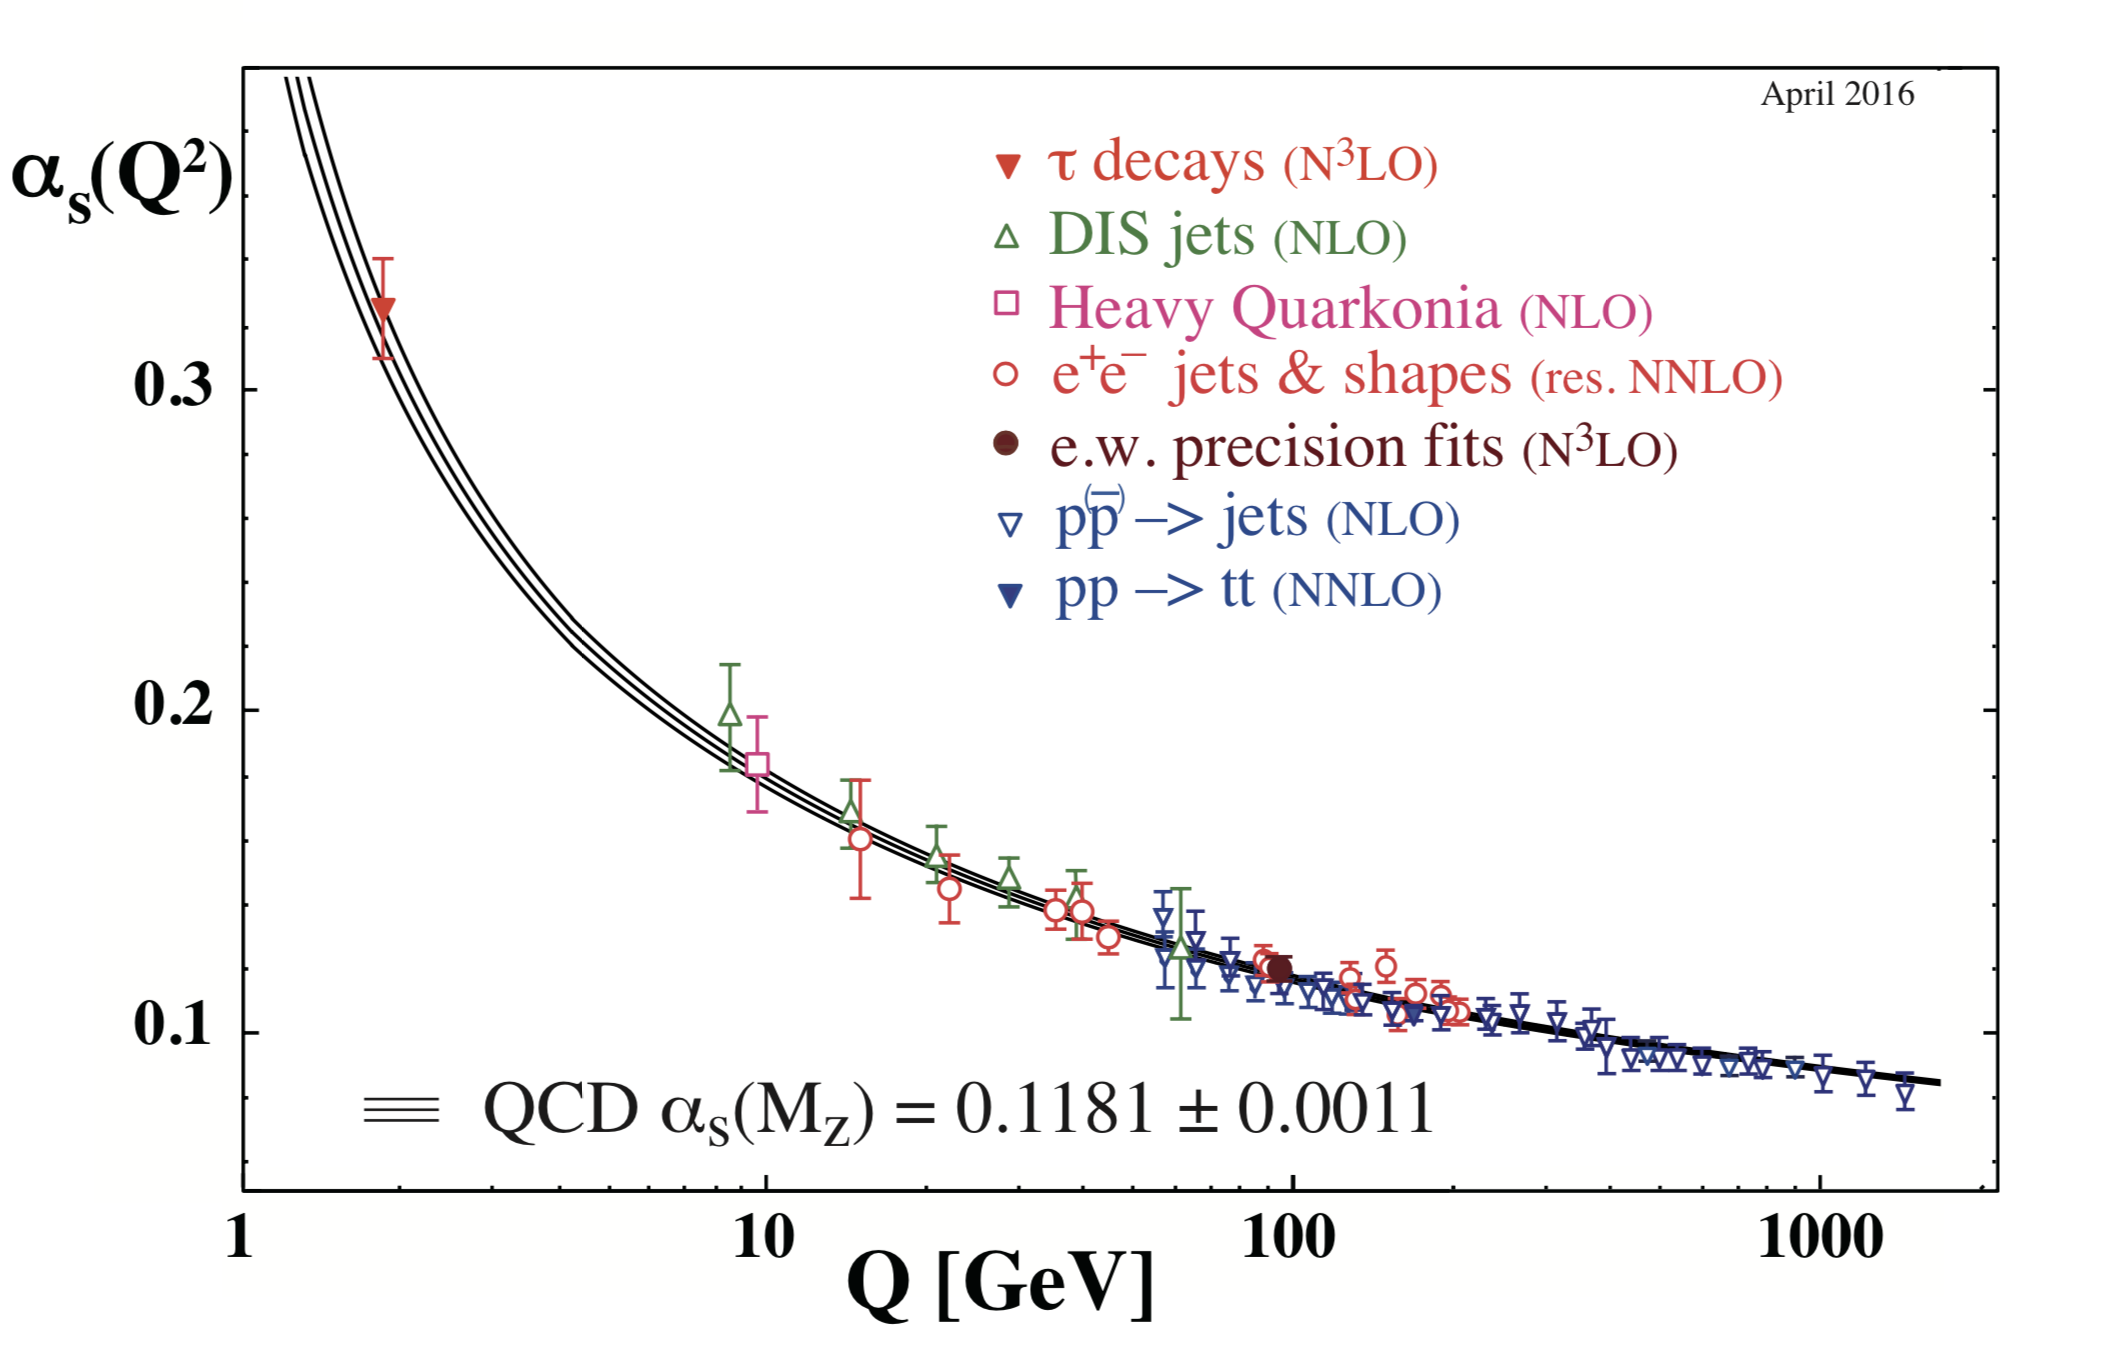
\includegraphics[width=0.8\textwidth]{gfx/alpharun}
	\caption{Summary of measurements of $\alpha_{s}$ as a function of the energy scale $Q$ \cite{pdg}.}
	\label{fig:alpharun}
\end{figure}

In QCD, the perturbative approach used to calculate the elements of the scattering matrix (pQCD), is 
possible only for high $Q^{2}\ $ processes ($Q^{2} \gg \mu^{2}$, thus $\alpha_{s} \ll 1$).
As already mentioned, in low transferred momentum processes $\alpha_{s}$ diverges. 
Therefore, it is impossible to express the elements of the scattering matrix in terms of power series
expansion of the strong coupling constant.
In this regime the evaluation of the Green’s functions of the QCD Lagrangian is possible
on a space-time lattice with spacing a, as proposed in 1974 by Wilson \cite{lattice}.
The aforementioned model, called lattice QCD (lQCD) gives the determination of the extrapolation to the continuum 
($a \rightarrow 0$) and it produces results to be compared with the experiments.

%
%
\section{States of hadronic matter}
\label{sec:1.2}

One of the interesting consequences of the running coupling constant is the possibility of having
different states of the hadronic matter. The state is essentially determined by the mean transferred 
momentum in the interactions which define the value of $\alpha_{s}$. 
A system with low mean transferred momentum is in the \textit{confinement} regime, therefore quarks
and gluons are required to be confined in hadrons. Otherwise for systems characterised by a high mean transferred momentum,
the \textit{asymptotic freedom} regime allows the formation of a plasma where quarks and gluons are
essentially free. This state of matter is called Quark Gluon Plasma (QGP) and it is supposed to be the same state in which the
universe was in the first microseconds after the Big Bang.
One of the main goals of the HENP is the study of the phase transitions between the different
states of the hadronic matter.

Considering a system with finite dimensions, composed by hadronic matter, it can be useful to describe it 
using thermodynamical variables like temperature $(T)$ and chemical potential $(\mu)$. In this
specific framework the chemical potential is interpreted as the energy required to create a 
baryonic state and it is called baryon chemical potential $(\mu_{B})$. 
Figure \ref{fig:qgpdiagram} shows the phase diagram of the QCD matter predicted by the theory and 
the values of temperature $T$ and baryon chemical potential $(\mu_{B})$ which are accessible
experimentally in high energy heavy ion collisions.

\begin{figure}
    \centering
    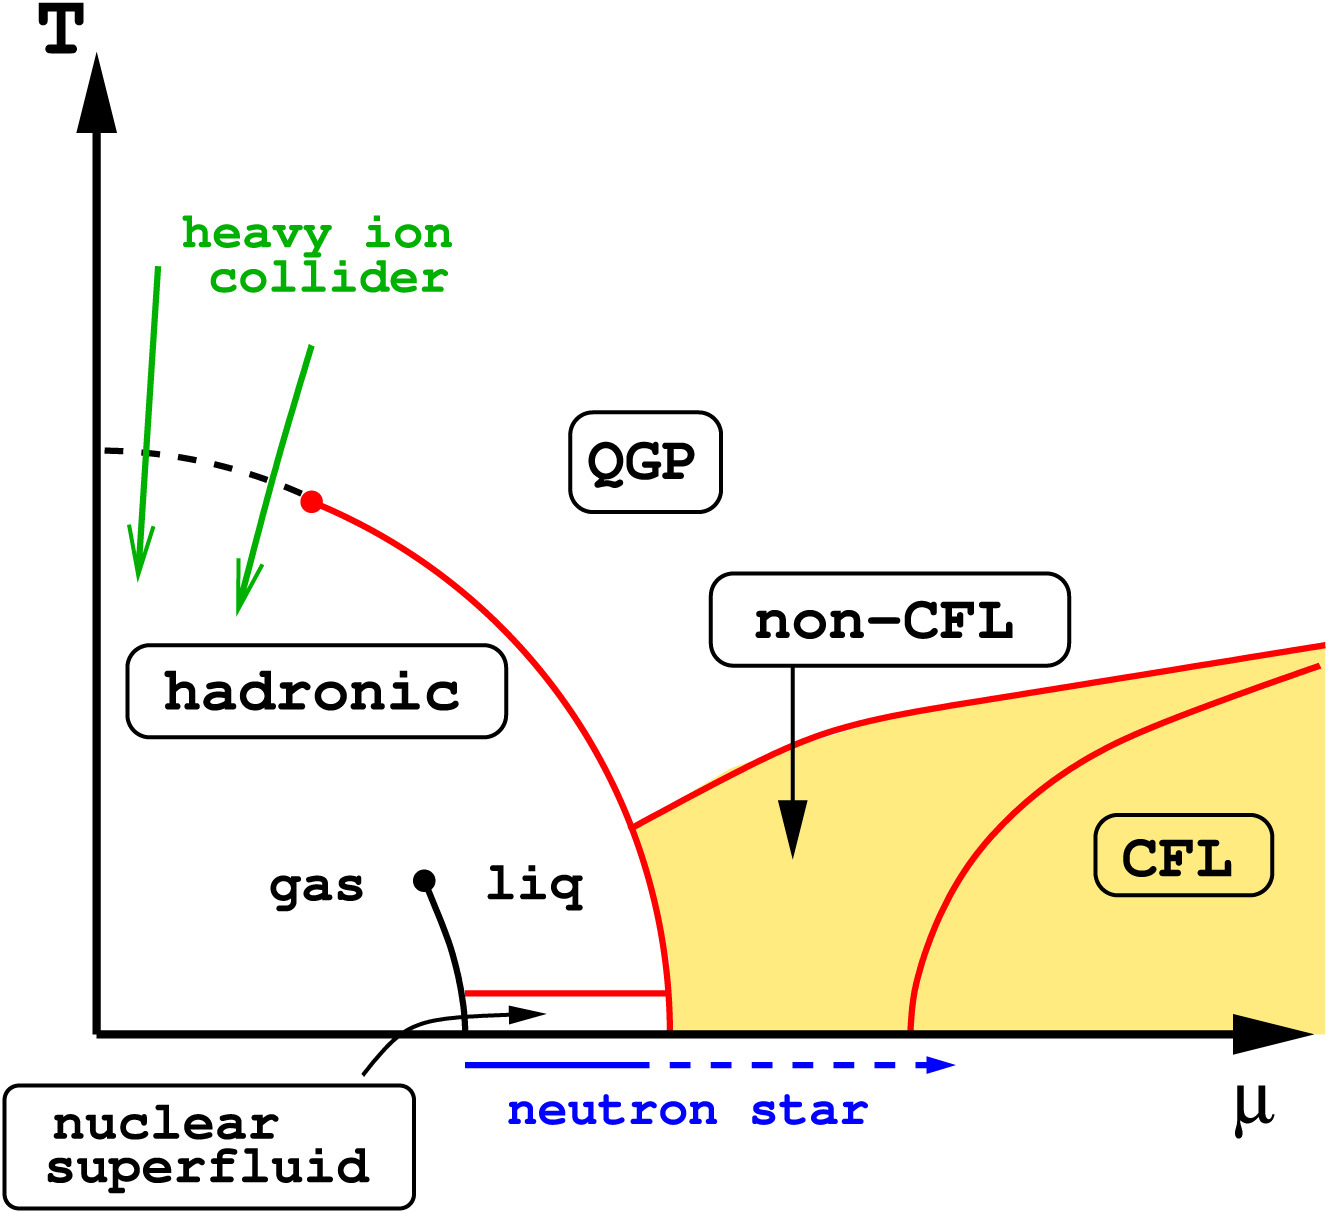
\includegraphics[width=0.6\textwidth]{gfx/qgpphase}
	\caption{Schematic representation of the nuclear matter phase diagram from \cite{qgpphase}. QGP refers to the Quark Gluon Plasma state, CFL (Colour-Flavour Locked) corresponds to the colour superconducting phase that is present in systems with high baryon chemical potential. The green arrows represent the phase space investigated by collider experiments at the Relativistic Heavy Ion Collider (RHIC) and at the Large Hadron Collider (LHC).}
	\label{fig:qgpdiagram}
\end{figure}

The origin of the diagram (T$=\mu_{B}=0$ GeV) corresponds to the QCD vacuum. At T$=0$ GeV, $\mu_{B}$ is 
the energy required to create a baryonic state, therefore ordinary matter (proton, neutrons and nuclei)
sits around $1$ GeV on the $\mu_{B}$ axis. Along the $\mu_{B}$ axis one can find the phase transition to a state,
the Color Superconducting Phase, that has been predicted to be present in matter at high density,
e.g. in  the core of neutron stars \cite{csp}.
Along the T axis, where $\mu_{B}=0$, there is a phase transition when T$\ \gg \Lambda_{\mathrm{QCD}}$. 
At this temperatures the average momentum exchange between quarks and gluons is so high that they reach
the \textit{asymptotic freedom}, hence they are no longer confined in colour singlets states.
In these conditions they constitute a plasma of free coloured partons, similar to the primordial 
universe: the aforementioned QGP.

The order of the phase transition is determined by the behavior of the derivatives of the system free energy
with respect to the time. It basically describes how fast the free energy varies in a
neighborhood of the transition temperature.
A first order transition takes place when a latent heat is present, leading to a discontinuous free
energy first derivative and a variation of the entropy.
If no latent heat is involved in the process, a second order transition occurs. For this kind of transitions the free energy 
first derivative is continuous, while higher order derivatives of the free energy are 
discontinuous.
When the transition occurs with a continuous behavior of the free energy and its derivatives,
it is called a \textit{crossover} transition.
In $\mu_{B}=0$ conditions, the transition from hadron gas to the QGP takes place when T $\approx 150$ MeV
with a \textit{crossover} transition.

%
%
\section{Heavy Ion Collisions}
\label{sec:1.3}

The QCD phase diagram is derived by theories and models, but their predictions are difficult to test.
For the T $\approx0$ GeV and high $\mu_{B}$ region, important suggestions can come from astronomic observations 
of neutron stars. 
For high T regions, instead, the only known way to cross the phase boundary between ordinary hadronic matter
and QGP is by colliding ultrarelativistic heavy ions in the laboratory.

The journey of the High Energy Nuclear Physics started in the '70s at the Lawrence Berkeley National Laboratory
where the first experiments with heavy ions collisions (HIC) were performed at modestly relativistic conditions 
($\approx 2\ $ GeV/nucleon).
In 1986, two HIC experiments started simultaneously at the Super Proton Syncrotron (SPS) at CERN and at the
Alternate Gradient Syncrotron (AGS) at Brookhaven, colliding Oxygen ions on fixed target at higher energies.
Nowadays the two main hadron colliders that are carrying out a HIC program with dedicated experiments are the
Relativistic Heavy Ion Collider (RHIC) at the Brookhaven National Laboratory (BNL) and the Large Hadron
Collider (LHC) at CERN.

%
\subsection{The "Little Bang" at the LHC}
\label{sec:1.3.1}

Atomic nuclei are composite systems of nucleons with finite dimensions. When they collide at 
ultrarelativistic energies the problem of the description of the collision, that can be very
complex, arises.
The Glauber Model \cite{glauber} is a semi-classical model that describes nucleus–nucleus 
interaction in terms of nucleon–nucleon (NN) interactions.
The Glauber Model is based on the assumption of the \textit{optical limit} which translates in the following hypotheses:
\begin{itemize}
    \item nucleons are point like and independent inside the nuclei;
    \item only hadronic interactions are considered: protons and neutrons cannot be distinguished;
    \item the collision does not deflect colliding nucleons: they travel in a straight line;
    \item the cross section for an elementary nucleon-nucleon interaction is constant during the whole 
    process.
\end{itemize}
Under this assumption the Glauber Model allows a quantitative calculation of the interaction
probability, the number of elementary NN collisions ($\mathrm{N}_{coll}$), the number
of the participants nucleons ($\mathrm{N}_{part}$) and the extension of the overlap region.
These quantities are expressed in terms of the impact parameter $\vec{b}$, which characterizes
the collisions geometry.
A direct experimental measurement of the impact parameter is precluded and the same is for
$\mathrm{N}_{coll}$ and $\mathrm{N}_{part}$.
However, the Glauber Model allow us to correlate these variables with measurable quantities
such as the total number of particles produced in the collision.

\begin{figure}[!h]
    \centering
    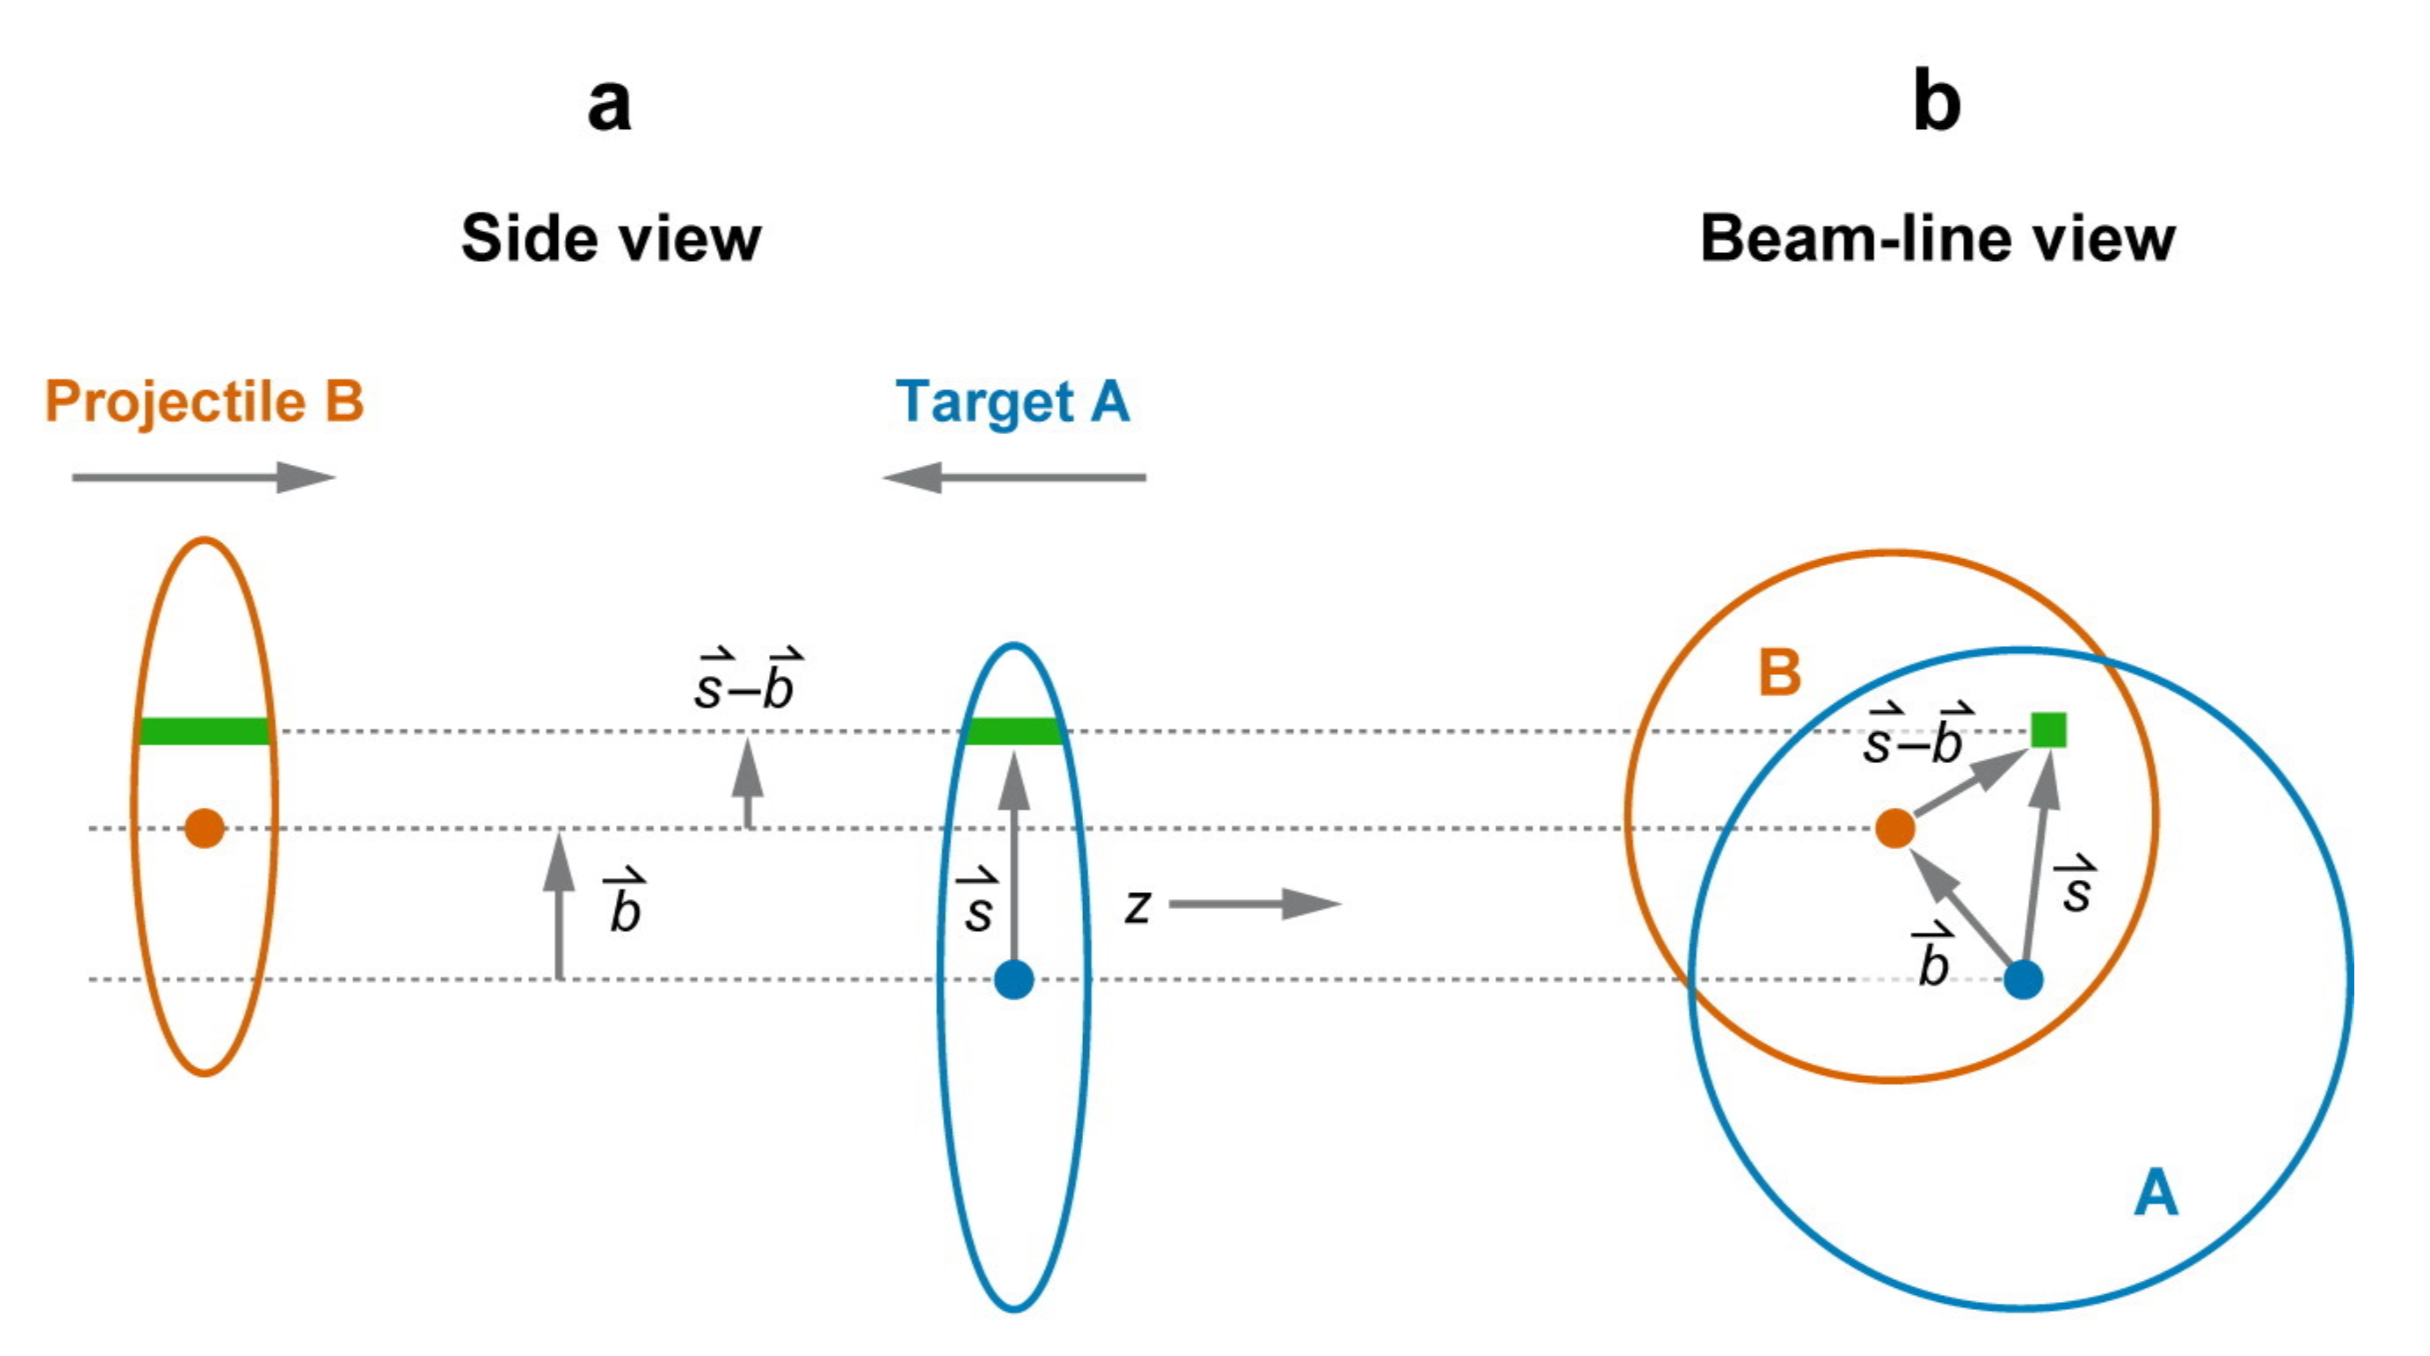
\includegraphics[width=0.8\textwidth]{gfx/glauber}
	\caption{Sketch of the longitudinal and transverse view of an heavy ion collision taken from \cite{glauber}. In the side view (a), the colliding nuclei are squeezed to represent the Lorentz boost contraction due to their momentum.}
	\label{fig:glauber}
\end{figure}

Following the notation introduced in Figure \ref{fig:glauber} the nuclear overlap function for two colliding
nuclei (A and B) can be written as:
\begin{equation} \label{eq:overlap}
    T_{AB}(\vec{b}) = \int T_{A}(\vec{s})\,T_{B}(\vec{s}-\vec{b}) \mathop{d^{2}s}
\end{equation}
and represents the probability of finding a nucleon inside the 
overlap region of the two colliding nuclei, in the transverse plane.
$T_{A}(\vec{s})$ and $T_{B}(\vec{s}-\vec{b})$ are the \textit{thickness functions} for the nucleus A and B, respectively.
They represent the probability of finding a nucleon in the unit transverse area located at 
$\vec{s}\xspace$, given the probability per unit volume $\rho(\vec{s},z)$:
\begin{equation} \label{eq:thickfunc}
    T(\vec{s}) = \int \rho(\vec{s},z) \mathop{dz}.
\end{equation}
Taken into account the model assumptions, only binary interactions between nucleons are considered and the interaction does not
deflect the trajectory of the interacting nucleons.
Therefore, each nucleon can participate in more than one binary collision. 
The probability of having $n$ binary collisions between the nuclei A and B, having A and B nucleons
respectively, can be computed using the binomial statistics as follows:
\begin{equation} \label{eq:ABprob}
    P(n,\vec{b}) = \frac{AB!}{n! (AB-n)!}[T_{AB}(\vec{b})\sigma_{inel}]^{n} [1-T_{AB}(\vec{b})\sigma_{inel}]^{AB-n}.
\end{equation}
From this expression the total inelastic cross section is obtained as a function of the impact
parameter integrating the double differential cross section for two colliding nuclei:
\begin{equation} \label{eq:doublediff}
    \frac{d^{2} \sigma^{AB}_{inel}(b)}{\mathop{db^{2}}} = \sum_{n=1}^{AB} P(n,b)
    = 1 - [1-T_{AB}(\vec{b})\, \sigma_{inel}]^{AB}
\end{equation}
\begin{equation}
    \sigma^{AB}_{inel}(b) = \int_{0}^{\infty} 2 \pi \, b \mathop{db} \,
    [1 - [1-T_{AB}(\vec{b})\, \sigma_{inel}]^{AB}]
\end{equation}


From eq. \ref{eq:ABprob}, $\mathrm{N}_{coll}$ can be derived as a function of the impact parameter 
summing all the possible numbers of collisions weighted by their own probability and using the
definition of the mean of the binomial distribution:
\begin{equation} \label{eq:ncoll}
    \mathrm{N}_{coll}(b) = \sum_{n=1}^{AB} n\, P(n,b) \ = AB\, T_{AB}\, \sigma_{inel}.
\end{equation}
Similarly $\mathrm{N}_{part}$ can be obtained by integrating over $\vec{s}$ the contribution of the
projectile nucleus and the contribution of the target nucleus as follow:
\begin{equation} \label{eq:npart}
    \mathrm{N}_{part}(b) = \int \mathop{d^{2}s} \, \bigl\{ A\, T_{A}(\vec{s})[1-(1- T_{B}(\vec{b}-\vec{s})\, \sigma_{inel})^{B}
    ] + B\, T_{B}(\vec{b}-\vec{s}) [1-(1-T_{A}(\vec{s})\,\sigma_{inel})^{A}] \bigr\}
\end{equation}
In eq. \ref{eq:ncoll} and \ref{eq:npart}, $\vec{b}$ has been replaced with its norm as the direction 
of the vector is relevant for polarized nuclei only.

In spite of its simplicity, the Glauber Model allows to express $\mathrm{N}_{coll}$ and 
$\mathrm{N}_{part}$ starting from $\rho(\vec{s})$ and $\sigma_{inel}$. The main limitation of the model is the usage of continuous density functions that implies to consider discrete physical quantities 
as continuous.

%
\subsection{Space time evolution of Heavy Ion collisions} \label{sec:1.3.2}

When two ultrarelativistic atomic nuclei collide, high hadron density and high temperatures
are produced in the impact region. 
In these experimental conditions a long lived and strongly interacting system is created.
The evolution of such a system, as well as the characterization of its properties, is very important
to improve our understanding of the Strong interaction. Hence it is one of the main subject of 
investigation of HI experiments.

\begin{figure}
    \centering
    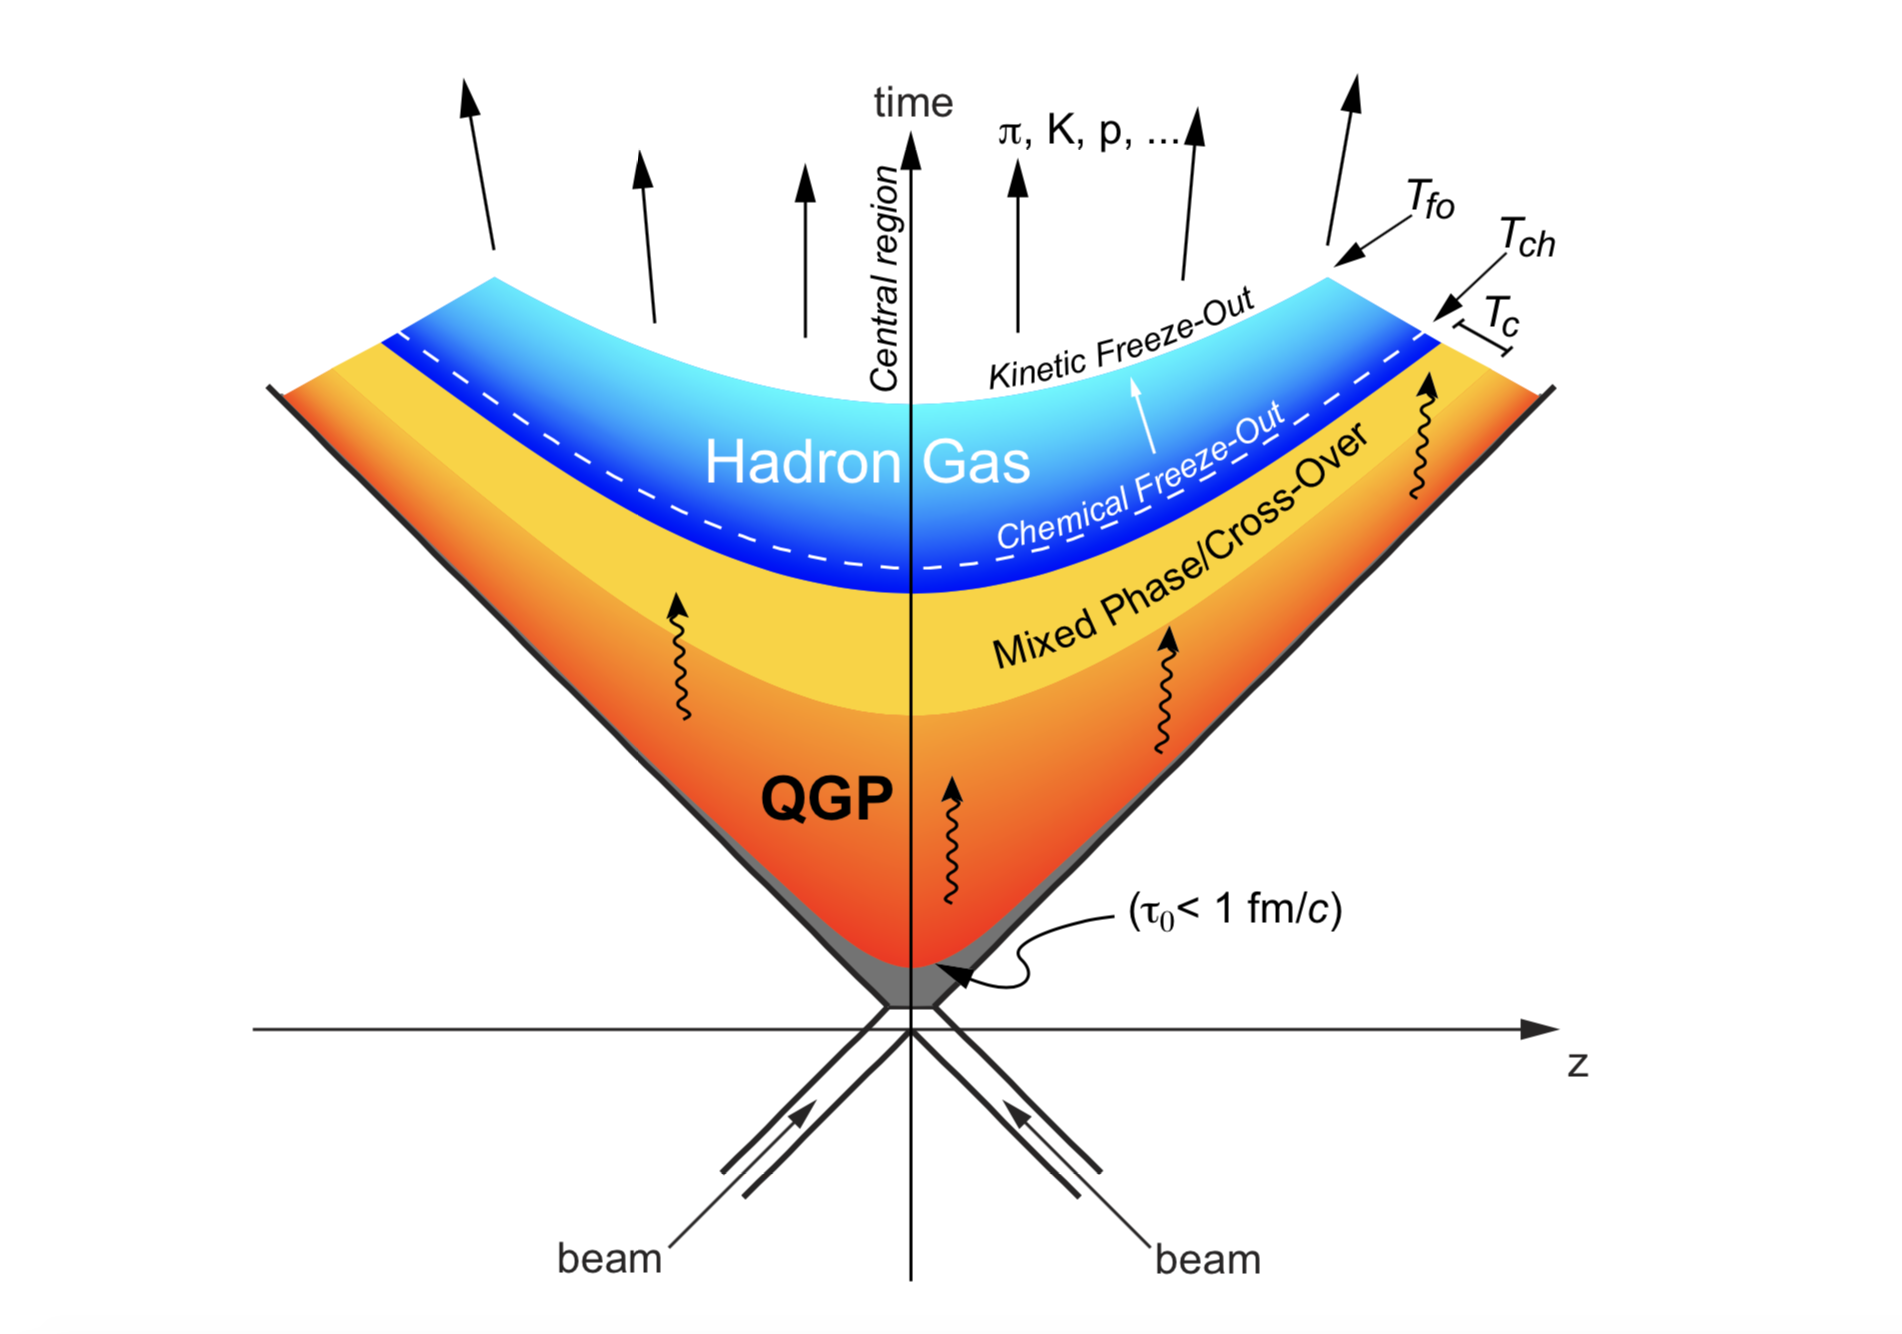
\includegraphics[width=0.9\textwidth]{gfx/evolution}
    \caption{Space-time representation of the evolution of the system created in a central Heavy Ion collision in the mid-rapidity region. The z direction is parallel to the beam line.}
	\label{fig:evolution}
\end{figure}

The space-time evolution of the system, produced in a HI collision, proceeds through different phases.
The current view on this evolution is summarized in Figure \ref{fig:evolution} and in the following the features of the system in different time ranges are reported:
\begin{enumerate}
    \item \textbf{\textit{t < 0} fm/\textit{c}:} the two atomic nuclei travel in the beam line. In modern accelerators
        the nuclei are strongly Lorentz contracted in the beam line direction since they are at almost the speed of 
        light (factor of 2700 at the LHC);

    \item \textbf{\textit{t = 0} fm/\textit{c}:} collision time. The geometry of the collision can be described using the Glauber Model reported in the previous section;

    \item \textbf{\textit{0 < t}} $\, \pmb{\lesssim \, \text{\Large$ \tau_{0} $} \sim }$ \textbf{\textit{1} fm/\textit{c}:}
            in the early collision stages hard processes (i.e. process with high transferred momentum $Q^{2}$) occur between
            colliding partons. In this phase called \textit{pre–equilibrium}, all the particles with high mass or/and
            high momentum are produced. In high energy collisions, as those provided at the LHC, the nuclei constituent partons 
            lose their energy in the mid-rapidity\footnote{The rapidity is defined by Eq. \ref{eq:rapidity} in Section 
            \ref{sec:3.2}.} region ($y\approx 0$) and then they escape at forward rapidities ($|y| \gg 0$). 
            The escaping valence quarks bring the baryonic potential, carried by the colliding nuclei, at forward rapidity thus vanishing the baryon chemical potential at mid-rapidity.
            The resulting system is a hot and dense medium. If the energy density is high enough, as at the LHC, a 
            transition to the QGP state is expected.
            After a short strong parton rescattering phase, the obtained droplet of QGP matter reaches the equilibrium
            at his proper time $\tau_{0}$;
            
    \item \textbf{\textit{1}} $\, \pmb{\lesssim}$ \textbf{\textit{t}} $\, \pmb{\lesssim}$ \textbf{\textit{10} fm/\textit{c}:}
            the QGP droplet reach the thermal equilibrium and it collectively expands under the thermal pressure
            gradients generated at the system boundaries. Relativistic hydrodynamics models \cite{relhydro} are commonly 
            used to describe the rapid expansion of the QGP matter, providing useful insights to interpret the 
            experimental data.
            As a consequence of the expansion, the system cools down and the energy density decreases, transiting eventually
            from the Quark Gluon Plasma phase to the ordinary hadronic matter;

    \item \textbf{\textit{10}} $\, \pmb{\lesssim}$ \textbf{\textit{t}} $\, \pmb{\lesssim}$ \textbf{\textit{15} fm/\textit{c}:}
            the critical temperature between the two phases is reached. At this temperature the hadronization process
            starts, leading the system into an interacting \textit{hadron resonance gas}. At this stage, the expansion
            and the cooling of the system continue, meanwhile elastic and inelastic interactions among the hadrons
            occur. 
            When the energy density is decreased that much to not allowing inelastic interactions, the relative 
            abundances of different particle species are fixed. The temperature at which the system stops to 
            interact inelastically is called temperature of \textit{chemical freeze-out} T$_{ch}$. After the
            \textit{chemical freeze-out} only elastic processes took place, varying the particles momentum.
            When elastic interactions ends as well, the particles momentum spectra are fixed and this occurs
            at the temperature of \textit{kinetic freeze-out} T$_{kin}$;

    \item \textbf{\textit{t}} $\, \pmb{\gtrsim}$ \textbf{\textit{15} fm/\textit{c}:} hadrons created in 
            the collision escape the interaction region with no further interactions. This regime is 
            also known as \textit{free hadron stream}.
\end{enumerate}

The particles produced in the collisions and escaped from the interaction region are detected by 
the experimental apparata carrying information about the environment in 
which they have been produced and about the medium in which they have travelled. 
In the following it will be shown how properties of the systems and characteristics of its 
evolution can be inferred by the measurement of particle production spectra and particle correlations.

%
%
\section{Nuclei production in Heavy Ion collisions} \label{sec:1.4}

The main subject of this thesis is the study of the \dst dibaryon production at the LHC energies.
Except for the deuteron, dibaryons are little known objects. In the next chapter, more details
on what dibaryons are and the description of our understanding about dibaryons, will be provided. 

The (anti-)nuclei are loosely bound objects and it is not trivial to describe how they can emerge from Heavy Ion collisions. 
The following sections are dedicated to a brief description of the two main classes of models
that try to explain the nuclei and anti–nuclei production mechanism in HI collisions: the Statistical 
hadronization Models (SHMs) and the Coalescence model \cite{deuprod}.
The production of dibaryons and in particular \dst \ \ -- which can be considered as an excited deuteron -- \ is supposed to be driven by the same mechanism responsible for the (anti-)nuclei production.

%
\subsection{Statistical hadronization Models} \label{sec:1.4.1}

The Statistical hadronization Models (also known as Thermal Models) were successfully developed
in order to describe the abundances of different particle species produced in the collision 
between particles.

The general idea behind these models is that the final state of the interaction is composed by
all the particle states compatible with the conservation laws imposed by the underlying theory 
of interaction (in our case the Standard Model of particle physics). 
The relative abundance of different particle states is set by the maximisation of the total phase
space filled by the system, to which each particle species contributes according to its partition 
function. These models are of particular interest in HI collisions as the presence of an expanding 
medium that eventually reaches the thermal equilibrium seems appropriate for the statistical
hadronization approach. 

The system created in a relativistic HIC is large enough to be modelled using the Grand Canonical
ensemble. 
This formalism can be used as the central rapidity region is in equilibrium with a thermal reservoir 
(the rest of the medium created in a HI collision) and quantities like energy, baryon number, 
charge and isospin are conserved on average. Most of the barrel experiments (as for ALICE central
detectors) measure only this part of the phase space, hence the use of the Grand Canonical formalism 
is allowed.
Within this formalism the parameters describing the equilibrium condition of a HIC
include the temperature T and the baryon chemical potential $\mu_{B}$. On this basis 
the partition function of the system can be written as:
\begin{equation} \label{eq:partfunction}
    Z(T,V,\mu) = \Tr \Big[ e^{-\beta(H-\Sigma_{i}Q_{i}\mu_{i})} \Big]
\end{equation}
with
\begin{equation}
    \mu = \sum_{i} Q_{i} \mu_{Q_{i}} \ \ \ \mathrm{and} \ \ \ \beta = \frac{1}{T}
\end{equation}
where $V$ is the volume of the system at equilibrium, $H$ is the
Hamiltonian and $\mu_{Q_{i}}$ is the chemical potential associated to the conserved quantum number
$Q_{i}$.
For a strongly interacting medium, the main conserved quantum numbers are the electric charge $Q$,
the strangeness content of the system $S$ and the baryon number $B$.
The Hamiltonian $H$ in the partition function is that one of a Hadron Resonance Gas since it is able 
to describe the behavior of a strongly interacting medium reproducing over a wide temperature range
the equation of state obtained with lQCD calculations before the transition to a deconfined state.
The choice of the mesonic, baryonic and resonance states included in the Hamiltonian depends on the
implementation of the model and it determines the maximum temperature that can be described accurately.

The partition function of the system is the product of the contribution of all the particle states
in the Hadron Resonance Gas:
\begin{equation} \label{eq:partfuncprod}
    Z(T,V,\mu) = \prod_{i} Z_{i}(T,V,\mu_{i}) \ \ \ \rightarrow \ \ \ 
    \log Z(T,V,\mu) = \sum_{i} \log Z_{i}(T,V,\mu_{i}).
\end{equation}
The partition functions are defined by the spin–statistics theorem:
\begin{equation} \label{eq:partfuncspin}
    \log Z_{i}(T,V,\mu_{i}) = \frac{V g_{i}}{2 \pi^{2}} \int_{0}^{\infty}\
     \pm p^{2} \mathop{dp} \, \log \Big[1\pm \lambda_{i}(T,\mu_{i})e^{- \beta \epsilon_{i}} \Big]
\end{equation}
where Bose-Einstein distribution for bosons are indicated as ($+$) and the Fermi-Dirac distribution for fermions are those obtained by using ($-$).
The $g_{i}$ constant is the degeneracy state $i$ and $\epsilon_{i}$ is the energy of one 
particle of the species $i$ with momentum $p (\epsilon_{i} = \sqrt{p^{2} + m_{i}^{2}})$.
The dependence on the chemical potentials is encoded within the \textit{fugacity}
$\lambda_{i}$:
\begin{equation} \label{eq:fugacity}
    \lambda_{i}(T,\mu_{i}) = e^{\beta(B_{i}\mu_{B} + S_{i}\mu_{S} + Q_{i}\mu_{Q})}
    = e^{\beta \mu_{i}}
\end{equation}
where $B_{i}$, $S_{i}$ and $Q_{i}$ are the baryon number, the strangeness content and the electric
charge associated with the particle species and $\mu_{B}$ , $\mu_{S}$ and $\mu_{Q}$ are the 
respective chemical potentials. As described in \cite{pbmstat}, expanding the logarithm and
integrating over the momentum, the partition function for the species $i$ becomes:
\begin{equation}
    \log Z_{i}(T,V,\mu_{i}) = \frac{V T g_{i}}{2 \pi^{2}}
    \sum_{k=1}^{\infty} \frac{(\pm 1)^{k+1}}{k^{2}} \lambda^{k}_{i} m_{i}^{2} K_{2}(\beta k m_{i})
\end{equation}
where the ($+$) is for bosons, the ($-$) for fermions and the $K_{2}$ is the second 
kind modified Bessel function of second order.

The average number of particle for the species $i$ for a system described by the Gran
Canonical ensemble, is defined as:
\begin{equation} \label{eq:particleyields1}
    \langle N_{i} \rangle ^{th} (T,V,\mu_{i}) = \frac{1}{\beta} \frac{\partial}{\partial \mu_{i}}
    \log Z_{i}(T,V,\mu_{i})
    \frac{V T g_{i}}{2 \pi^{2}}
    \sum_{k=1}^{\infty} \frac{(\pm 1)^{k+1}}{k} \lambda^{k}_{i} m_{i}^{2} K_{2}(\beta k m_{i}).
\end{equation}
This equation does not fully describe the particle abundances measured in HI collisions.
For the measured yields one needs to consider the feed–down contributions from all the other
particle species (resonances) $j$ in the thermal system that can decay strongly in a final
state containing particles of the species $i$:
\begin{equation} \label{eq:particleyields2}
    \langle N_{i} \rangle ^{th} (T,V,\mu) = \langle N_{i} \rangle ^{th} (T,V,\mu_{i})
    + \sum_{j} \Gamma_{j \to i} \langle N_{j} \rangle ^{th} (T,V,\mu_{j})
\end{equation}
where $\Gamma_{j \to i}$ is the decay rate of the state $j$ into the final state $i$.

The definition of particle yields is valid in the limit of a low density system, 
where the repulsion interaction between the hadrons constituting the systems is negligible.
The treatment of these interactions is still matter of active theoretical research. Nevertheless 
Eq \ref{eq:particleyields2} and \ref{eq:particleyields1} already indicate the crucial 
dependencies of the observed particle yields on the
temperature $T$, volume $V$ and the chemical potentials $\mu_B$, $\mu_Q$ and $\mu_S$.

In Heavy Ions collisions no net strangeness is present in the colliding nuclei, thus 
$\mu_S = 0$, and $\mu_Q$ is fixed by the isospin asymmetry in the collision.
Therefore two of the five parameters of the model are constrained by the collisions
conditions.
The baryon chemical potential $\mu_B$ is not constrained as the "amount of baryonic number"
transported in the equilibrium region depends on the energy of the collision.
The dependence on the volume $V$ of the system can be removed looking at ratio between 
the yields of different particle species, which therefore depends only on the temperature 
of the system and on the baryon chemical potential.
\begin{figure} 
    \centering
    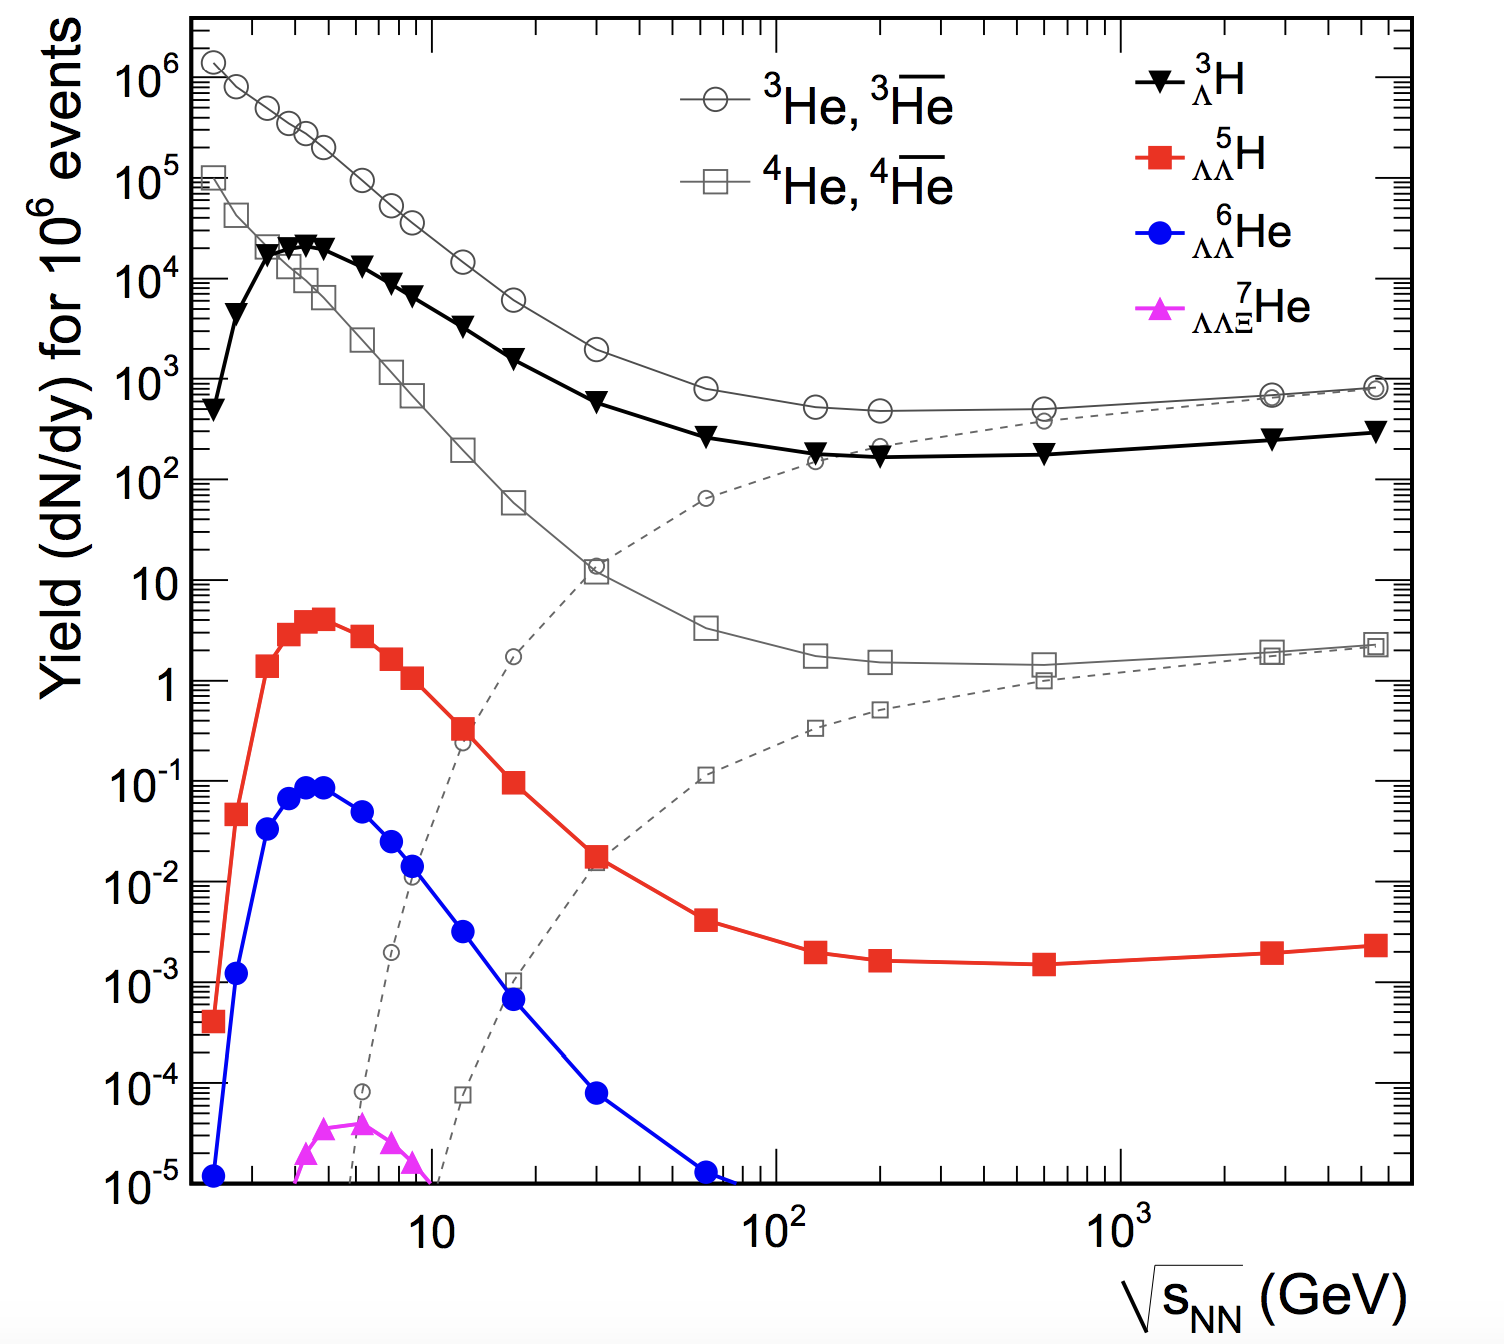
\includegraphics[width=0.7\textwidth]{gfx/yields}
    \caption{Thermal model predictions for the production of various nuclei, anti-nuclei and hyper–nuclei as a function of the ion collision energy taken from \cite{yields}. At low collision energy the baryon chemical potential differs significantly from zero and the particle yield favours matter over anti–matter. As the energy increases, $\mu_{B}$ decreases and this difference vanishes.
}
\label{fig:aliceyields}
\end{figure}
In the framework of the thermal models, light nuclei yields arise naturally when the chemical 
freeze–out temperature and the baryon chemical potential are set.
A possible explanation on how the light nuclei can survive to the high temperature of the chemical 
freeze–out was pointed out in \cite{yields}: as the system expansion after the chemical freeze–out
is supposed to conserve the entropy density, such conservation could be the steering mechanism for 
the nuclei production. From the fit of the particle abundances at lower energies, the 
authors of \cite{yields} predicted, using the thermal model, the yields of (anti-)nuclei 
at the LHC energy \ref{fig:aliceyields}.

%
\subsection{Coalescence Models} \label{sec:1.4.2}

Coalescence models \cite{deuprod} represent a different theoretical approach developed to explain 
the measured light nuclei production in Heavy Ions collisions. 
These models address the problem assuming that light nuclei are created at the kinetic freeze-out. 
They are static models and there is no attempt to give a detailed description of the 
interactions that lead to their formation.
The fundamental idea behind these predictions is that if nuclei constituents are close enough in 
phase space at the kinematic freeze-out they can bind to form a nucleus. 
The coalescence models make a prediction about the momentum distribution of the produced light 
nuclei as a function of the production spectra of the constituents.

The first coalescence model was developed to describe the deuteron formation in
proton-nucleus collisions in 1961 and in the following years it has been extended to 
the production of various light nuclei in nucleus-nucleus collisions.
The momentum spectrum for the $i$ species is linked to the proton momentum spectrum,
which is used as a proxy of the constituent spectrum, by using the following equation:
\begin{equation}
    E_{i} \frac{d^{3}N_{i}}{\mathop{dp_{i}^{3}}} = B_{A} \Big( E_{p} \frac{d^{3}N_{p}}{\mathop{dp_{p}^{3}}} \Big)^{A}.
\end{equation}

The proton spectrum is assumed to be identical to that one of the constituent neutron.
One of the main reasons for this generalization is that proton spectra are easier to measure
in an experiment.
These nucleon spectra are not those measured in the experiments, but the ones produced in the 
collision and not yet modified by the coalescence mechanism.
The coalescence parameter $B_{A}$ is interpreted as a function of the radius $p_{0}$, that 
is the maximum distance at which coalescence can happen.
In the simplest formulation of the coalescence models only the momentum space is considered
(not the space-time), thus the coalescence parameter can be expressed neglecting the spin:
\begin{equation} 
    B_{A} = \Big( \frac{4}{3}\, \pi \,p_{0}^3 \Big)^{A-1} \frac{m_{i}}{m_{p}^{A}}.
\end{equation}
where $p_{0}$ is the aforementioned radius and $m_{i}$ and $m_{p}$ are the nucleus and proton
mass, respectively.

More sophisticated versions of this model predict a dependence on the geometry of the system
and rely on different constituents momentum spectra and different formulation of 
the coalescence parameter $B_{A}$. Nevertheless, thanks to its simplicity and the presence
of one single parameter $p_{0}$, the most commonly used coalescence approach, for the comparison with the experimental data, is
the simple one which has been briefly shown above.
